\documentclass[12pt]{article}
\usepackage[left=3cm, top=3cm, right=3cm, bottom=3cm]{geometry}
\usepackage[utf8]{inputenc}      % accents dans le source
\usepackage[T1]{fontenc}
\usepackage[french]{babel}
\usepackage{graphicx}
\usepackage{graphics}
\usepackage{amsmath}
\usepackage{tikz}
\usepackage{xcolor} 
\usepackage{mathtools}
\usepackage{parskip}
\usepackage{subcaption}
\usepackage[export]{adjustbox}
\usepackage{chemist}

\title{\textbf{TP 1 - Électromagnétisme} \\ Électrostatique}
\author{MENARD Alexandre \\ VIEILLEDENT Florent}
\setlength{\parindent}{1cm}
\begin{document}
\maketitle

\section*{Introduction}
L'électrostatique est le domaine de l'électromagnétisme qui étudie les champs électrique permanent, qui ne dépendent pas du temps.
Dans ce travail pratique, on cherchera à vérifier plusieurs lois de l'électrostatique, notamment l'équation de Laplace et la formule pour la capacité d'un condensateur plan. 
Pour la première loi on mesurera le potentiel entre des électrodes circulaires et pour la deuxième on étudiera la décharge du condensateur avec un oscilloscope.

\break

\section{Potentiel électrostatique généré par des électrodes circulaire}
	Dans cette partie, on souhaite vérifier si l'équation de Laplace est valide dans le cadre de l'électrostatique. Pour cela, nous réaliserons des mesures de d.d.p
	dans l'espace entre électrodes circulaires concentriques pour les comparer au modèle théorique. 
	
	\subsection{Modèle}
	On se place dans le cadre d'un régime permanent où les électrodes sont à l'équilibre. Les charges se retrouvent donc à la surface des électrodes, d'où $\rho(M) = 0$, et ceux pour tout point $M$.
	L'équation de Laplace nous donne $\Delta V(M) = 0$, avec $\Delta V(M)$ l'opérateur Laplacien. 
	On se place dans un référentiel polaire (voir Fig1) dont l'origine est le centre de nos électrodes. Les électrodes étant circulaires, le système est invariant par rotation, donc $V(r,\theta)=V(r)$, on s'attend à des équipotentielles circulaire.
	
	% On est dans un régime permanent, les électrodes sont à l'équilibre. Il n'y a donc pas de charge entre les électrodes et l'équation de Laplace nous donne $\Delta V =0$, avec $\Delta V$ le laplacien du potentiel. On se place dans un référentiel polaire dont l'origine est le centre de nos électrodes. Les électrodes étant circulaire,le système est invariant par rotation, donc $V(r,\theta)=V(r)$, on s'attend à des équipotentielles circulaire. De plus, en utilisant l'expression du laplacien en polaires on obtient:
	
	\begin{figure}[!h]
		\begin{center}
			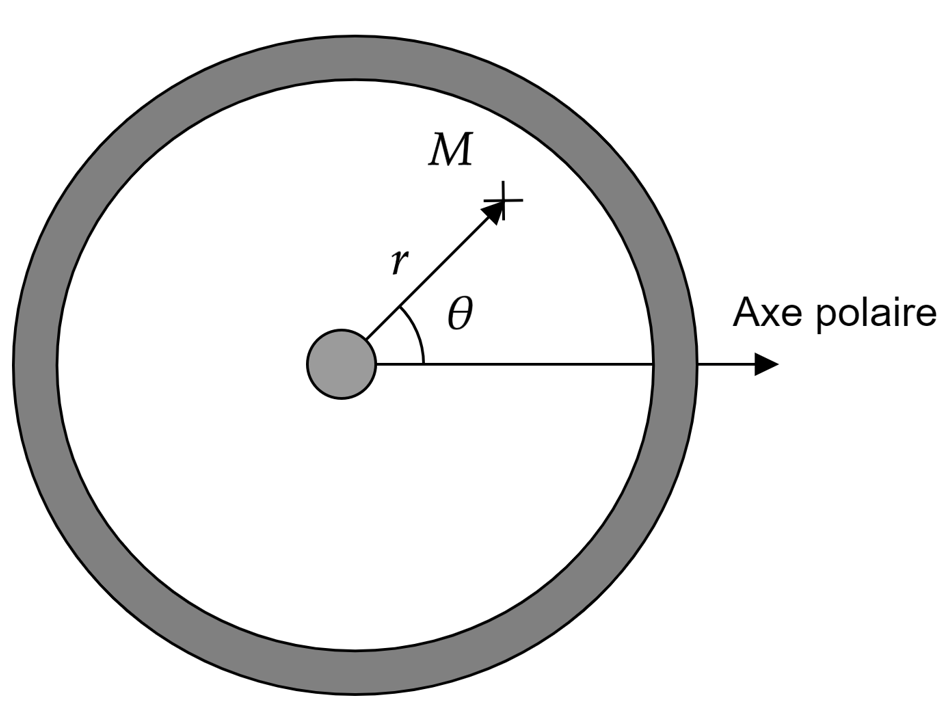
\includegraphics[scale=0.2]{img/schema.png}
			\caption{Schéma du système d'électrodes}
		\end{center}
	\end{figure}

	\begin{align*}
		\Delta V(M) = \frac{1}{r} \frac{\partial}{\partial r} \left( r \frac{\partial V(M)}{\partial r} \right) = 0 & \Rightarrow \frac{\partial V(M)}{\partial r} = \frac{C}{r} \\
		& \Rightarrow V(M) = C \ln(r) + V_0
	\end{align*}	
		
	$C$ et $V_0$ sont des constantes d'intégration qu'on détermine grâce aux conditions aux limites $V(R_1 = d)$ et $V(R_2 = d_{int})$ avec $d_{ext}$ le rayon de la petite électrode et $d_{int}$ le rayon interne de la grande électrode. Il vient alors:
	
	\begin{equation}
		V(r) = \frac{V(R_2) - V(R_1)}{ln(\frac{R_2}{R_1})} ln(\frac{r}{R_1}) + V(R_1)
	\end{equation}

	Pour le modèle, nous négligeons les variations de potentiel sur $z$, cependant les électrodes ne sont pas très hautes devant leurs rayons. Pour respecter cette limite, nous nous efforcerons de réaliser
	les mesures sur une même hauteur (en mesurant sur le papier carboné). Les mesures permettront de décider de l'impact de cette hypothèse sur le modèle.
	
	\subsection{Protocole expérimental}
	
	On fixe deux électrodes circulaire en aluminium sur du plastique isolant. L'électrode circulaire à un diamètre intérieur $d_{int}=160,0\pm 0.5 mm$ et un diamètre extérieur $d_{ext}=180,0\pm 0.5 mm$. L'incertitude sur les longueurs est données par la graduation de $1mm$ de notre règle. On peut choisir entre deux électrodes intérieurs différentes: une pleine de diamètre $d=15,0\pm 0.5 mm$ et une creuse de diamètre intérieur $d_{int}'=60,0\pm 0.5 mm$ et de diamètre extérieur $d_{ext}'=80,0\pm 0.5 mm$. \\ \\ 
	Ces électrodes sont reliées par des pinces crocodiles et des fils à une alimentation continue dont on a mesuré la tension $U_0= \pm V$ avec un  voltmètre. Pour mesurer le potentiel entre nos électrodes, on place du papier carbonée entre nos électrodes et le plastique isolant. Notre voltmètre est relié par une borne à l'électrode centrale et l'autre à une sonde qu'on place sur la papier carboné à l'endroit où on souhaite mesurer le potentiel. La coordonnées polaires de la sonde sont obtenues grâce à une webcam relié à un ordinateur et le logiciel ImageJ. On néglige le courant généré par le papier électrique sa conductivité étant faible devant celle des électrodes. \\ \\
	On commence par déterminer deux courbes d'équipotentielles pour $V_1=$ et $V_2=$, puis on mesure $V(r)$ pour différentes valeurs de r.  
	
	\subsection{Résultats et interprétation}
	
	
\section{Mesure de capacité de condensateurs plans}
	\subsection{Modèle}
La capacité $C$ d'un condensateur plan est donnée par $C=\epsilon_0\frac{S}{d}$ avec $\epsilon_0=8,85.10^{-12} F.m^{-1}$ la permittivité du vide, $d$ la distance entre les deux plaques et $S$ la surface des plaques. Cette formule est valables pour des plaques infinies ce qui correspond à $d\ll S$. \\

On peut utiliser la loi des mailles pour trouver une équation différentiel. On note V la tension aux bornes du condensateur. Lorsque le circuit, composé du condensateur et d'une , est ouvert, on a :
\begin{equation}
V-V_{res}=0
\end{equation}
On utilise la loi d'Ohm $V=RI$, la définition du courant $I=\frac{dQ}{dt}$ et la définition de la capacité $Q=CV$. On obtient une équation différentielle qu'on résout:
\begin{equation}
V-RC\frac{dV}{dt}=0 \Longleftrightarrow V=V_0exp(\frac{t}{RC}
\end{equation}
Dans notre cas $V_0=U_0$ la tension de l'alimentation et $R=R_{osc}$ la résistance de l'oscilloscope.
	
	\subsection{Protocole expérimental}
	
	\subsection{Résultats et interprétation}
	
\section*{Conclusion}	

\end{document}